\section{Bremsstrahlung and Migdal-type absorption}\label{sec:12.6}

A nucleus that is suddenly set moving is a charge that radiates. Besides leaving an electron--hole pair behind, in $6.1\times10^{-3}$ of the kicks for silicon at a recoil energy of \SI{100}{eV} (\cref{sec:12.3}), it emits photons, the bremsstrahlung of the recoil. Kouvaris and Pradler pointed out that such photons, unlike the recoil, are easy to see, and used them to carry xenon searches to lower masses~\cite{kouvaris2017probing}. A second process uses the same nonadiabatic structure with the roles of energy and momentum exchanged. A scalar coupled to nucleons and absorbed by a nucleus gives it almost no momentum but its whole rest energy, and the electrons, which do not follow the nucleus exactly, take that energy~\cite{dzuba2024migdal}. Both effects were worked out for isolated atoms. We will compute both in a crystal. For bremsstrahlung the crystal replaces the charge of the nucleus by a dynamical Born charge, which in silicon and germanium is fixed exactly by the measured dielectric function; for absorption it replaces the atomic photoabsorption cross-section by the loss function.

\subsection{Photon emission in a medium}\label{sec:12.6-photon}

The photon is a new final-state particle in this book, and \cref{app:C.16} sets up what we need: the transverse radiation field as a set of oscillators, its minimal coupling to charges, and the golden-rule rate of emitting one photon. A charge $e_{\mathrm{c}}$ at rest that is set moving with velocity $\vect{v} \ll 1$ in a time short compared with $1/\omega$ radiates the photon number spectrum \cref{eq:C.16-soft}, flat in energy. And inside a transparent medium of refractive index $n_r(\omega)$ the same current radiates $n_r$ times more, \cref{eq:C.16-medium}: the density of photon modes grows as $n_r^2n_{\mathrm{grp}}$, the field of one photon shrinks as $(n_rn_{\mathrm{grp}})^{-1/2}$, and the group index $n_{\mathrm{grp}}$ cancels. Together,
\begin{equation}
  \frac{\dd N_\gamma}{\dd\omega_\gamma} = n_r(\omega_\gamma)\,\frac{2\alpha}{3\pi}\,\frac{e_{\mathrm{c}}^2}{e^2}\,\frac{v^2}{\omega_\gamma} ,
  \label{eq:12.6-classical}
\end{equation}
with $\omega_\gamma$ the energy of the photon. The spectrum holds for photon wavelengths long compared with the emitter, the dipole limit, and for a medium that does not absorb at $\omega_\gamma$, so that the photon is a propagating mode.

A nucleus in an atom does not radiate with its bare charge. Its electrons are pulled along, and the photon sees the dipole of the whole atom. Kouvaris and Pradler computed this in second-order perturbation theory, kick and emission in both orders, and found the bare spectrum, $e_{\mathrm{c}} = Z_\kappa e$ in \cref{eq:12.6-classical}~\cite[Eq.~(3)]{kouvaris2017probing}, with $Z_\kappa^2$ replaced by $|f(\omega_\gamma)|^2$~\cite[Eq.~(8)]{kouvaris2017probing}. Their $f$ is the atomic scattering factor, and in our units it is fixed by the dipole polarizability $\alpha_{\mathrm{pol}}(\omega)$ of the atom,
\begin{equation}
  Z^*_{\mathrm{at}}(\omega) \equiv f(\omega) = -\frac{m_e\omega^2}{e^2}\,\alpha_{\mathrm{pol}}(\omega) ,
  \label{eq:12.6-atom}
\end{equation}
the free-atom limit of the dynamical Born charge of \cref{sec:12.6-brems}. A model of electrons bound to the nucleus by springs shows what it means. If the nucleus moves by $u$ at frequency $\omega$, an electron with natural frequency $\omega_n$ follows with the amplitude $\omega_n^2u/(\omega_n^2 - \omega^2)$, and the atom acquires the dipole $-eu\sum_nf_n\omega^2/(\omega_n^2 - \omega^2)$, with $f_n$ the oscillator strengths, which sum to $Z_\kappa$ (\cref{sec:4.3}). At high frequency the electrons stay behind and the dipole is $Z_\kappa eu$, the bare charge. At low frequency they follow, the neutral atom carries no dipole, and $Z^*_{\mathrm{at}}$ falls as $\omega^2$. For silicon, with the static polarizability of $37.3$ atomic units~\cite{schwerdtfeger2019table}, that is $4\pi\times37.3\,a_0^3 = \SI{69.5}{\angstrom^3}$ in Heaviside--Lorentz units, $Z^*_{\mathrm{at}} = -0.050$ at \SI{1}{eV}: a photon of an electronvolt sees one twentieth of an electron charge.

\subsection{Crystal nuclear-recoil bremsstrahlung}\label{sec:12.6-brems}

In a crystal the charge that moves with a displaced nucleus is the Born effective charge of \cref{sec:5.5}. The Born charge is defined for slow displacements, with the electrons following adiabatically. A photon of an electronvolt oscillates faster than the lattice but not much slower than the electrons. What it sees is the \emph{dynamical Born charge} $Z^*_\kappa(\omega)$: the dipole created per unit displacement of one nucleus of species $\kappa$ oscillating at frequency $\omega$, all other nuclei at rest, at zero macroscopic field, with the electrons responding at $\omega$. By the Maxwell relation \cref{eq:5.5-Z}, taken at frequency $\omega$, it is also the force on the nucleus per unit field. At $\omega \to 0$ it is the Born charge $Z^*_\kappa$, at $\omega$ far above every electronic frequency it is $Z_\kappa$, and for a free atom it is $Z^*_{\mathrm{at}}$ of \cref{eq:12.6-atom}. The nucleus couples to the macroscopic field of a photon, $\vect{\mathcal{E}}_\gamma$, through the term of \cref{eq:5.5-HE} at that frequency,
\begin{equation}
  H_\gamma = -e\sum_I\vect{u}_I\cdot Z^*_\kappa(\omega_\gamma)\cdot\vect{\mathcal{E}}_\gamma .
  \label{eq:12.6-Hgamma}
\end{equation}
The local fields at the nucleus are inside $Z^*_\kappa$, and $\vect{\mathcal{E}}_\gamma$ is the field of the medium's photon mode of \cref{app:C.16}.

\emph{The amplitude.} Dark matter kicks nucleus $I$ with $K = \ee^{\ii\vect{q}\cdot\vect{X}_I}$, and the photon is emitted by $D = -e\vect{u}_I\cdot Z^*_\kappa\cdot\langle1_\gamma|\vect{\mathcal{E}}_\gamma|0\rangle$, which acts on the nucleus only. The process has two time orders. With $H$ the Hamiltonian of the crystal, $|i\rangle$ and $|f\rangle$ its initial and final states and $|n\rangle$ the intermediate ones, the second-order amplitude is
\begin{equation*}
  A_{fi} = \sum_n\Bigl[\frac{\langle f|D|n\rangle\langle n|K|i\rangle}{\omega_\gamma - (E_n - E_f)} - \frac{\langle f|K|n\rangle\langle n|D|i\rangle}{\omega_\gamma + (E_n - E_i)}\Bigr] .
\end{equation*}
When $\omega_\gamma$ is large compared with the energy differences in the denominators, we expand in their ratio. At zeroth order the two terms give $\langle f|[D,K]|i\rangle/\omega_\gamma$, which vanishes, since $\vect{u}_I$ and $\ee^{\ii\vect{q}\cdot\vect{X}_I}$ commute. At first order, closure turns the energy differences into commutators with $H$, and
\begin{equation*}
  A_{fi} = -\frac{1}{\omega_\gamma^2}\,\langle f|\bigl[[H,D],K\bigr]|i\rangle .
\end{equation*}
Whatever potential holds the nucleus, it is a function of the positions, so $[H,\vect{u}_I] = -\ii\vect{P}_I/M_\kappa$, and $[\vect{P}_I,\ee^{\ii\vect{q}\cdot\vect{X}_I}] = \vect{q}\,\ee^{\ii\vect{q}\cdot\vect{X}_I}$. The double commutator is the kick times $\ii e\,(\vect{q}/M_\kappa)\cdot Z^*_\kappa\cdot\langle1_\gamma|\vect{\mathcal{E}}_\gamma|0\rangle$, and the amplitude factorizes into the matrix element of the kick and the emission amplitude of a charge $eZ^*_\kappa$ that jumps to the velocity $\vect{v}_N = \vect{q}/M_\kappa$. This is the classical result of \cref{app:C.16} for a sudden kick, and the lattice potential has dropped out. The neglected terms are of relative order $(E_n - E_i)/\omega_\gamma$. The displacement $\vect{u}_I$ changes the number of phonons by one, so the energies in question are phonon energies, and the expansion holds for $\omega_\gamma \gg \omega_{\mathrm{ph}}$: the nucleus moves freely during one period of the photon.

Each kick of nucleus $\kappa$ thus comes with the photon spectrum \cref{eq:12.6-classical} for the charge $eZ^*_\kappa(\omega_\gamma)$ and the velocity $\vect{v}_N$. Inserting the kick into \cref{eq:8.2-spectrum} with the joint response of \cref{sec:12.1-def}, and the photon energy as a third energy deposited, gives the rate.
\begin{keyresult}[Crystal nuclear-recoil bremsstrahlung]
For photon energies $\omega_{\mathrm{ph}} \ll \omega_\gamma$ below the absorption edge of the crystal, and momentum transfers above the zone, where the kicks of different nuclei add incoherently,
\begin{equation}
  \begin{split}
  \frac{\dd^2\mathcal{R}}{\dd\omega_l\,\dd\omega_\gamma} = \frac{1}{\rho_T}\,\frac{\rho_\chi}{\mchi}\int\dd^3v\,f_\chi(\vect{v})\int\frac{\dd^3q}{(2\pi)^3}\sum_\kappa\,
  &\underbrace{\mathfrak{D}_{\kappa\kappa}(\vect{q},\vect{v})\,S_{\kappa\kappa}(\vect{q},\omega_l)}_{\text{kick}} \\
  &\times\underbrace{\frac{2\alpha\,n_r(\omega_\gamma)}{3\pi\,\omega_\gamma}\,\frac{|Z^*_\kappa(\omega_\gamma)\cdot\vect{q}|^2}{M_\kappa^2}}_{\text{photons per kick}}\,\delta(\omega_l + \omega_\gamma - \omega_{\vect{q}}) ,
  \end{split}
  \label{eq:12.6-brems}
\end{equation}
with $S_{\kappa\kappa}(\vect{q},\omega_l)$ the lattice response of \cref{chap:11} in whatever regime it is, single phonons, multiphonons or free recoil. At a cubic site $|Z^*_\kappa\cdot\vect{q}|^2 = Z^{*2}_\kappa q^2$.
\end{keyresult}
\noindent For a gas of atoms, $n_r = 1$, $Z^*_\kappa \to Z^*_{\mathrm{at}}$ and a free recoil, \cref{eq:12.6-brems} is the rate of Kouvaris and Pradler~\cite[Eq.~(8)]{kouvaris2017probing}; with the bare charge $Z_\kappa$ in place of $Z^*_\kappa$ it is their bare-nucleus rate~\cite[Eq.~(3)]{kouvaris2017probing}. Note that their derivation kept only the elastic atomic channel, the atom left in its ground state, and the crystal formula does the same: the electrons appear only through $Z^*_\kappa(\omega_\gamma)$.

The photon must be soft, its momentum $n_r\omega_\gamma$ small compared with $q$, which for photons of an eV and momentum transfers of keV holds by three orders of magnitude. The wavelength must be long compared with the cell, which makes $Z^*_\kappa$ the zone-center quantity. The impulse approximation, $E_R \gg \omega_{\mathrm{ph}}$, is not needed, since the lattice potential dropped out of the amplitude. Below the zone, however, the kicks of neighboring nuclei interfere, and the photon sees the dipole of a whole cell. For a coupling to nucleon number the cell is pushed as a unit. Its dipole is then accelerated only through the small difference of nucleon number per mass between its atoms, the cancellation that \cref{we:8-nucleon} found for optical phonons. Above the absorption edge the photon is absorbed before it leaves the crystal. The same amplitude then makes an electron--hole pair. That piece is the exchange of a transverse photon between the moving nucleus and the electrons, a correction to the Coulomb amplitude of the Migdal effect (\cref{sec:12.1}) suppressed by powers of the velocities of the charges. The photon pole is bremsstrahlung, and the continuum is Migdal ionization; nothing is counted twice.

\emph{The dynamical Born charge of silicon and germanium.} What remains is $Z^*_\kappa(\omega)$, and one exact sum rule fixes much of it. Let every nucleus of the crystal move together, by $\vect{u}(t) = \vect{u}\,\ee^{-\ii\omega t}$. In the frame that moves with the nuclei, the electrons see the clamped crystal plus the inertial force $-m_e\ddot{\vect{u}} = m_e\omega^2\vect{u}$ on each electron, a uniform force indistinguishable from a uniform field $\vect{\mathcal{E}}_{\mathrm{in}} = -m_e\omega^2\vect{u}/e$. At zero macroscopic field the electrons respond to $\vect{\mathcal{E}}_{\mathrm{in}}$ as to an applied field, with the polarization $[\varepsilon(\omega) - 1]\vect{\mathcal{E}}_{\mathrm{in}}$, local fields included, and $\varepsilon(\omega)$ the electronic dielectric function at clamped nuclei. A rigid translation of the neutral cell adds no dipole of its own, so this polarization is the whole dipole per cell, $\Omega\vect{P} = e\sum_\kappa Z^*_\kappa(\omega)\cdot\vect{u}$. Hence
\begin{equation}
  \sum_\kappa Z^*_\kappa(\omega) = -\frac{\Omega\,m_e\,\omega^2}{e^2}\,\bigl[\varepsilon(\omega) - 1\bigr] ,
  \label{eq:12.6-sum}
\end{equation}
with $\Omega$ the cell volume. At $\omega \to 0$ the right-hand side vanishes, the neutrality of the Born charges \cref{eq:5.5-neutral}. At $\omega$ above every electronic frequency, $\varepsilon - 1 \to -\omega_p^2/\omega^2$ with the plasma frequency of all $N_e$ electrons of the cell, $\omega_p^2 = e^2N_e/(\Omega m_e)$, and the sum tends to $N_e = \sum_\kappa Z_\kappa$, the bare charges. For a dilute gas, $\varepsilon - 1$ is the density of atoms times $\alpha_{\mathrm{pol}}$, and \cref{eq:12.6-sum} becomes \cref{eq:12.6-atom}. The two atoms of silicon or germanium are exchanged by the inversion through the bond center, so their dynamical Born charges are equal at every frequency, and
\begin{equation}
  Z^*(\omega) = -\frac{\Omega\,m_e\,\omega^2}{2e^2}\,\bigl[\varepsilon(\omega) - 1\bigr]
  = -\frac{N_{\mathrm{v}}}{2}\,\bigl[\varepsilon(\omega) - 1\bigr]\frac{\omega^2}{(\omega_p^{\mathrm{val}})^2}
  \qquad (\text{Si, Ge}) ,
  \label{eq:12.6-ZSi}
\end{equation}
with $N_{\mathrm{v}} = 8$ valence electrons per cell and the valence plasma frequency $\omega_p^{\mathrm{val}}$ of \cref{sec:10.2}. No calculation of the phonon response is needed: the measured refractive index gives the dynamical Born charge.

Below the gap $\varepsilon$ changes slowly, and $Z^*(\omega) \simeq -C_\kappa\omega^2$ with $C_\kappa = \Omega m_e(\varepsilon_\infty - 1)/2e^2$, the coefficient of the small-$\omega$ expansion that \cref{app:E.17} specifies. For silicon, with $\Omega = \SI{40.05}{\angstrom^3}$ and $\varepsilon_\infty = 11.7$, $C_\kappa = \SI{0.155}{eV^{-2}}$; with the measured dielectric function at \SI{1}{eV}, $\varepsilon = 12.37$~\cite{franta2017temperature}, $Z^*(\SI{1}{eV}) = -0.165$. The photons per kick then grow as $\omega_\gamma^3$, and the rate is suppressed by $\omega_\gamma^4$ against that of a nucleus with a fixed charge. The suppression is that of the free atom, but the crystal is a stronger emitter. The polarizability per atom of the solid, $\Omega(\varepsilon - 1)/2 = \SI{228}{\angstrom^3}$ at \SI{1}{eV}, is 3.3 times that of the free atom, \SI{69.5}{\angstrom^3}. The emission goes as the square of the charge, $3.3^2 = 10.7$, and the photon gains $n_r = 3.5$ on top. Per photon the silicon crystal emits 33 to 38 times more than its atoms between 0.3 and \SI{1}{eV}, and germanium, with $\varepsilon_\infty = 16.0$~\cite{li1980refractive}, 86 to 96 times more between 0.3 and \SI{0.65}{eV}. A free-atom estimate is therefore not an upper bound for the crystal.

\emph{Polar crystals.} In GaAs the Born charge is $Z^* = 2.11$ at zero frequency (\cref{we:5-lst}), and nothing suppresses the emission at small $\omega_\gamma$. The sum rule \cref{eq:12.6-sum} fixes the sum of the two dispersions, $Z^*_{\mathrm{Ga}}(\omega) - Z^* + Z^*_{\mathrm{As}}(\omega) + Z^*$, from the electronic dielectric function, but not their difference. That difference is a mixed response to a field and a displacement at frequency $\omega$, which frequency-dependent density-functional perturbation theory computes with shifted Sternheimer equations at $\pm\omega$ and a scissor to the measured gap, checked against \cref{eq:12.6-sum} and the static Born charge (\cref{app:E.17}), where each dispersion is also bounded by $|Z^*_\kappa(\omega) - Z^*_\kappa(0)| \le 0.9\,(\omega/\SI{1}{eV})^2$. We split the sum equally between the two sites and carry the bound as a band. The rate depends on the difference only through the cross term with $Z^*$, and below \SI{0.3}{eV} the band is a few percent wide.

\begin{figure}[tbp]
  \centering
  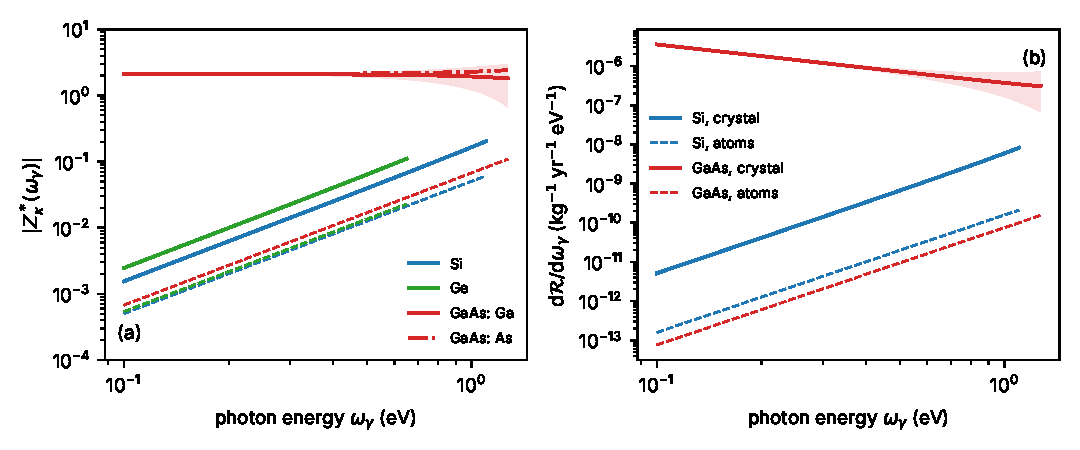
\includegraphics[width=\linewidth]{figures/ch12/fig12_5.pdf}
  \caption{Nuclear-recoil bremsstrahlung in silicon, germanium and GaAs below their absorption edges. (a) The dynamical Born charge $|Z^*_\kappa(\omega_\gamma)|$ against the photon energy (solid; dash-dotted for the arsenic site), from the sum rule \cref{eq:12.6-sum} with measured refractive indices: silicon at \SI{300}{K}~\cite{franta2017temperature} (0.1--\SI{1.1}{eV}), germanium at \SI{293}{K}~\cite{li1980refractive} (0.1--\SI{0.65}{eV}) and GaAs at \SI{295}{K}~\cite{skauli2003improved,polyanskiy2024refractiveindex} (0.1--\SI{1.27}{eV}, the range of the dispersion formula; its phonon term removed from the electronic $\varepsilon$). GaAs: $Z^* = 2.11$ at zero frequency and the dispersion of the sum split equally between the sites; shaded, the range allowed by the bound $|Z^*_\kappa(\omega) - Z^*_\kappa(0)| \le 0.9\,(\omega/\SI{1}{eV})^2$. Dashed: the free atoms, \cref{eq:12.6-atom} with the static polarizabilities 37.3 (Si), 40 (Ge) and 50 (Ga) atomic units~\cite{schwerdtfeger2019table}. (b) Rate per unit photon energy for $\mchi = \SI{100}{MeV}$, a heavy mediator coupled to nucleon number, $\sigma_p = 10^{-38}\,\mathrm{cm}^2$, the halo of \cref{sec:1.2}, \cref{eq:12.6-brems} with a free recoil. Solid: crystals; dashed: the same nuclei with the free-atom charges and $n_r = 1$; shaded: the GaAs band of panel (a).}
  \label{fig:12-brems}
\end{figure}

\Cref{fig:12-brems} shows the result. In GaAs the photons per kick are almost flat in $\ln\omega_\gamma$, as for a bare charge; half of them lie below \SI{0.36}{eV}. In silicon and germanium the spectrum climbs as $\omega_\gamma^3$ up to the absorption edge. The absolute numbers are small. A recoil of \SI{100}{eV} emits $4.0\times10^{-13}$ photons between 0.1 and \SI{1.1}{eV} in silicon and $1.7\times10^{-10}$ between 0.1 and \SI{1.27}{eV} in GaAs, against the Migdal probability of $6.1\times10^{-3}$ in silicon at the same recoil. At \SI{100}{MeV} the GaAs rate in panel (b) integrates to $9\times10^{-7}$ events per kilogram-year, and the silicon rate to $2\times10^{-9}$, while the Migdal rate of silicon with the same coupling is 30 (\cref{sec:12.3-rate}). The photons of GaAs lie below the gap, where the Migdal effect is closed, but they come with a Migdal signal above the gap that, judged by silicon, is larger by more than seven orders of magnitude. Bremsstrahlung in these crystals is therefore a check of the theory, not a search channel. At photon energies of hundreds of eV and above, where Kouvaris and Pradler found the reach of their xenon search, $\varepsilon \to 1$, the crystal emits as its atoms, and \cref{eq:12.6-sum} returns the bare charges as the electrons fall behind.

\begin{workedexample}{The GaAs enhancement over the atomic rate}\label{we:12-gaas}
How much more does a GaAs crystal radiate than a gas of the same atoms? We work at $\omega_\gamma = \SI{1}{eV}$ and then over the transparent band.

\emph{The dynamical Born charges.} The cell volume is $\Omega = a^3/4 = \SI{44.80}{\angstrom^3}$ with the static-lattice constant $a = \SI{5.638}{\angstrom}$ of \cref{tab:E-functionals}, the cell of the computed phonons and Born charge of \cref{sec:5.5}, and $\Omega m_e/e^2 = \SI{3.249e-2}{eV^{-2}}$. The dispersion formula of Skauli and collaborators~\cite{skauli2003improved}, as tabulated in Ref.~\cite{polyanskiy2024refractiveindex}, gives $n_r = 3.4185$ at \SI{1}{eV}, and without its phonon term the electronic dielectric function $\varepsilon = 11.688$. By \cref{eq:12.6-sum} at $\omega = \SI{1}{eV}$ the sum of the charges is $-(3.249\times10^{-2})(10.688) = -0.347$. Split equally, $Z^*_{\mathrm{Ga}}(\SI{1}{eV}) = 2.11 - 0.174 = 1.936$ and $Z^*_{\mathrm{As}}(\SI{1}{eV}) = -2.11 - 0.174 = -2.284$, so that the sum of their squares is 8.965. For any other split the sum of squares is $2(2.11 + b)^2 + 2(0.174)^2$, with $b$ half the difference between the two dispersions; the band of \cref{fig:12-brems} carries the values of $b$ that the bound allows.

\emph{The free atoms.} With $\alpha_{\mathrm{pol}} = 50$ and 30 atomic units~\cite{schwerdtfeger2019table}, that is $4\pi\times50\,a_0^3 = \SI{93.1}{\angstrom^3}$ and \SI{55.9}{\angstrom^3} in Heaviside--Lorentz units, \cref{eq:12.6-atom} gives $Z^*_{\mathrm{at}} = -0.0675$ for gallium and $-0.0405$ for arsenic at \SI{1}{eV}, and the sum of squares is $6.20\times10^{-3}$.

\emph{Per photon.} The two nuclei have nearly the same nucleon number per mass and nearly the same $q^2/M_\kappa^2$ at a given recoil, so the ratio of \cref{eq:12.6-brems} to its atomic form is the ratio of $n_r\sum_\kappa Z^{*2}_\kappa$ to $\sum_\kappa Z^{*2}_{\mathrm{at},\kappa}$: $3.4185\times8.965/6.20\times10^{-3} = 4.94\times10^3$ at \SI{1}{eV}. The crystal emits five thousand times more. Of that, $n_r$ contributes 3.4 and the Born charge the rest.

\emph{Over the band.} The ratio grows toward small $\omega_\gamma$ as $\omega_\gamma^{-4}$, since the atomic charges fall as $\omega_\gamma^2$ and the crystal charges do not. Integrated with the weight $1/\omega_\gamma$ of \cref{eq:12.6-brems} from 0.1 to \SI{1.27}{eV}, $\int n_r\sum_\kappa Z^{*2}_\kappa\,\dd\omega_\gamma/\omega_\gamma = 75.4$ and $\int\sum_\kappa Z^{*2}_{\mathrm{at},\kappa}\,\dd\omega_\gamma/\omega_\gamma = 4.03\times10^{-3}$, a ratio of $1.87\times10^4$. The full rate at $\mchi = \SI{100}{MeV}$ gives $1.88\times10^4$, the same to the precision shown, because the kinematics hardly depends on photon energies so far below the kinetic energy of the dark matter.

\emph{Per recoil.} A gallium nucleus with $E_R = \SI{100}{eV}$ has $v_N^2 = 2E_R/M = 3.08\times10^{-9}$, and with $2\alpha/3\pi = 1.549\times10^{-3}$ it emits $1.7\times10^{-10}$ photons in the band. The enhancement over the atom is large, four orders of magnitude, but it multiplies a small number. Its uncertainty is the band of \cref{fig:12-brems}: the rate at \SI{100}{MeV} lies between \SI{-19}{\percent} and \SI{+25}{\percent} of its central value.
\end{workedexample}

\subsection{Migdal-type absorption of a scalar}\label{sec:12.6-absorption}

A scalar of mass \SI{1}{keV} from the halo, absorbed in silicon, deposits \SI{1}{keV} with a momentum of only $k = m_\phi v \approx \SI{1}{eV}$. If it couples to nucleons, the nucleus takes that momentum, and its recoil energy, $k^2/2M_\kappa$, is \SI{e-11}{eV}. The energy must go somewhere else, and it goes to the electrons. Dzuba, Flambaum and Samsonov computed this for atoms~\cite{dzuba2024migdal}. In the language of \cref{sec:12.2} it is a Migdal effect at the momentum $k$ instead of $q$. The exact center-of-mass separation \cref{eq:12.2-cm} turns the kick $\ee^{\ii\vect{k}\cdot\vect{X}}$ into a kick of the whole atom and the boost $\exp(-\ii\vect{k}_e\cdot\sum_e\vect{\rho}_e)$ of the electrons, with $\vect{k}_e = m_e\vect{k}/m_A$. At the dipole order of \cref{eq:12.2-dipole} the amplitude to excite the electrons to $\Psi_f$ is $-\ii k_e\langle\Psi_f|D_{\hat k}|\Psi_0\rangle$. What differs from scattering is the energy. The field supplies $\omega = m_\phi$, and the whole of it goes to the electrons, $\omega_e = m_\phi$, while the lattice receives nothing to the precision of interest.

\emph{The coupling.} A scalar coupled to protons and neutrons, $\mathcal{L} \supset \phi\,(g_{\phi pp}\,\bar pp + g_{\phi nn}\,\bar nn)$, couples to each nucleus coherently, as in \cref{eq:8.1-nuclear}, with the nuclear form factor equal to one at these momenta. The interaction is $H_\phi = -\phi\sum_\kappa c_\kappa n_\kappa(\vect{p}_\phi)$, the nuclear density row of \cref{sec:8.1-absorption} with
\begin{equation*}
  c_\kappa = Z_\kappa\,g_{\phi pp} + (A_\kappa - Z_\kappa)\,g_{\phi nn} , \qquad g^\phi_{n_\kappa} = -c_\kappa ,
\end{equation*}
the per-species weight $c_\kappa$ of \cref{sec:11.3}, which here carries the couplings themselves rather than their ratio to a reference coupling. For equal couplings, $c_\kappa = A_\kappa g_{\phi nn}$.

\emph{The acceleration form.} For an atom the center-of-mass separation is exact; in a crystal there is no atom to separate, and we need another route to the same amplitude. The equations of motion give it. Whatever the interactions, the potential energy $V$ of the crystal depends on the positions alone, so $[H,\vect{X}_I] = -\ii\vect{P}_I/M_\kappa$ and $[H,\vect{P}_I] = \ii\nabla_{\vect{X}_I}V$, and the double commutator is $[H,[H,\vect{X}_I]] = \nabla_{\vect{X}_I}V/M_\kappa$. Between eigenstates with $\omega_{fi} = E_f - E_i \neq 0$ this reads $\omega_{fi}^2\langle f|\vect{X}_I|i\rangle = \langle f|\nabla_{\vect{X}_I}V|i\rangle/M_\kappa$. Expanding the kick to first order in $\vect{k}$,
\begin{equation}
  \Bigl\langle f\Big|\sum_Ic_\kappa\ee^{\ii\vect{k}\cdot\vect{X}_I}\Big|i\Bigr\rangle = \frac{\ii}{\omega_{fi}^2}\sum_I\frac{c_\kappa}{M_\kappa}\,\vect{k}\cdot\langle f|\nabla_{\vect{X}_I}V|i\rangle + O(k^2) ,
  \label{eq:12.6-accel}
\end{equation}
the acceleration form of the amplitude. It is exact, at every order of the Born--Oppenheimer expansion. Its matrix element is minus the total force on nucleus $I$, from the electrons and the other nuclei, between the initial and final states. Between electronic states this is the derivative coupling of \cref{eq:5.1-dcoup}, and \cref{eq:12.6-accel} is the boost amplitude \cref{eq:8.6-boost} with $q$ replaced by $k$ and the excitation energy by $\omega_{fi}$. In scattering the boost is the first term of an expansion in the velocity of the nucleus. Here the momentum is so small that only the dipole term matters, and the equations of motion give it exactly.

\emph{Couplings proportional to mass.} Let $c_\kappa = \tilde cM_\kappa$ for every species, with one constant $\tilde c$. The potential depends only on differences of positions, so the gradients with respect to all particles sum to zero, $\sum_I\nabla_{\vect{X}_I}V = -\sum_j\nabla_{\vect{r}_j}V$, the sum over electrons: the total force on the nuclei is minus the total force on the electrons. The same double commutator for the electrons, with $m_e$ in place of $M_\kappa$, turns the right-hand side of \cref{eq:12.6-accel} into a dipole matrix element of the electrons, and
\begin{equation}
  \Bigl\langle f\Big|\tilde c\sum_IM_\kappa\ee^{\ii\vect{k}\cdot\vect{X}_I}\Big|i\Bigr\rangle = -\tilde c\,m_e\,\langle f|n_e(\vect{k})|i\rangle\,\bigl[1 + O(kr)\bigr] ,
  \label{eq:12.6-mass}
\end{equation}
with $r$ the size of the states involved. The physical reading is the equivalence principle. A field that couples to the mass of every particle cannot, at zero momentum, distinguish them: it pushes the center of mass and nothing else, and its matrix elements between different states start at order $k^2$. A coupling to the mass of the nuclei is the coupling to the total mass minus that to the electrons, and only the second term excites the crystal. It is the electronic counterpart of the cancellation by which a coupling proportional to mass excites no optical phonon (\cref{eq:11.8-Gamma}).

The scalar therefore acts on the electrons as a density coupling of strength $\tilde cm_e$. The absorption formula \cref{eq:8.2-abs} with $S_{ee} = (2k^2/e^2)L$, \cref{eq:4.4-SL}, the electron-density form that holds above the phonon band, gives the rate.
\begin{keyresult}[Migdal-type absorption in a crystal]
For a scalar whose couplings to the nuclei are proportional to their masses, $c_\kappa = \tilde cM_\kappa$, absorbed with momentum $\vect{p}_\phi$ and energy $\omega_\phi \simeq m_\phi$ above the phonon band,
\begin{equation}
  \varGamma_{\mathrm{abs}} = \frac{\tilde c^2m_e^2\,p_\phi^2}{e^2\,m_\phi}\,L(\vect{p}_\phi \to 0, m_\phi) , \qquad
  \mathcal{R} = \frac{\rho_\chi}{\rho_T}\,\frac{\tilde c^2m_e^2\langle v^2\rangle}{e^2}\,L(m_\phi) ,
  \label{eq:12.6-absrate}
\end{equation}
with $L = \Imag[-1/\varepsilon]$ the loss function at zero momentum and $\langle v^2\rangle$ the mean squared speed of the halo in the laboratory.
\end{keyresult}
\noindent For the halo of \cref{sec:1.2}, $\langle v^2\rangle^{1/2} = \SI{379}{km.s^{-1}}$. The spectrum is that of dark-photon absorption, whose rate is $(\rho_\chi/\rho_T)\zeta^2L(m_\phi)$ (\cref{sec:10.7}), with $\zeta^2$ replaced by $\tilde c^2m_e^2\langle v^2\rangle/e^2$. Everything \cref{sec:10.7} found about screening carries over: the scalar is absorbed with the loss function, not with the absorptive part $\varepsilon_2$, suppressed near the absorption peaks of silicon, where $|\varepsilon|^2$ is large, and enhanced at the plasmon. In silicon and germanium, with one species, every coupling to nucleons is proportional to the mass up to the isotopes, so \cref{eq:12.6-absrate} is the whole rate.

The atomic result is the dilute limit. For a gas, $|\varepsilon| \to 1$ and $L \to \varepsilon_2$, and the photoabsorption cross-section $\sigma_\gamma$ of one atom fixes $\omega\varepsilon_2 = \nd_{\mathrm{at}}\sigma_\gamma$, with $\nd_{\mathrm{at}}$ the density of atoms. Then $\varGamma_{\mathrm{abs}} = \nd_{\mathrm{at}}v\,\sigma_\phi$ with $\sigma_\phi = \tilde c^2m_e^2(p_\phi/m_\phi)\sigma_\gamma/e^2$, which for $\tilde c = g_{\phi nn}/m_p$ is the relation of Dzuba, Flambaum and Samsonov between scalar absorption and photoionization~\cite[Eqs.~(14), (17)]{dzuba2024migdal}. They cautioned that rates in solids could differ from the atomic estimate, and \cref{eq:12.6-absrate} says by how much. Applied to a crystal with the measured photoabsorption, which in a medium is $\nd_{\mathrm{at}}\sigma_\gamma = \omega\varepsilon_2/n_r$, the atomic formula uses $\varepsilon_2/n_r$ where the crystal has $\varepsilon_2/|\varepsilon|^2$. The ratio, $n_r/|\varepsilon|^2$, is the medium factor. Far above the absorption edges, $\varepsilon \simeq 1 - \omega_p^2/\omega^2$ with $\omega_p$ the plasma frequency of the electrons bound below $\omega$, so that $n_r \simeq 1 - \omega_p^2/2\omega^2$ and $|\varepsilon|^2 \simeq 1 - 2\omega_p^2/\omega^2$, and
\begin{equation}
  \frac{n_r}{|\varepsilon|^2} = 1 + \frac32\,\frac{\omega_p^2}{\omega^2} + O\Bigl(\frac{\omega_p^4}{\omega^4},\ \varepsilon_2^2\Bigr) .
  \label{eq:12.6-medium}
\end{equation}
For silicon at \SI{1}{keV}, with the twelve electrons per atom bound by less than \SI{1}{keV} and $\omega_p = \SI{28.8}{eV}$, this is $1 + 1.2\times10^{-3}$. Near the plasmon and the absorption peaks it is far from one.

\begin{limitbox}[Migdal-type absorption of a scalar][lim:12.6a]
$\sigma_\phi = g_{\phi nn}^2(m_e^2/m_p^2)(p_\phi/m_\phi)\,\sigma_\gamma/4\pi\alpha$ per atom, with $\sigma_\gamma$ the photoionization cross-section at $\omega = m_\phi$~\cite[Eqs.~(14), (17)]{dzuba2024migdal}.
\par\smallskip
{\centering
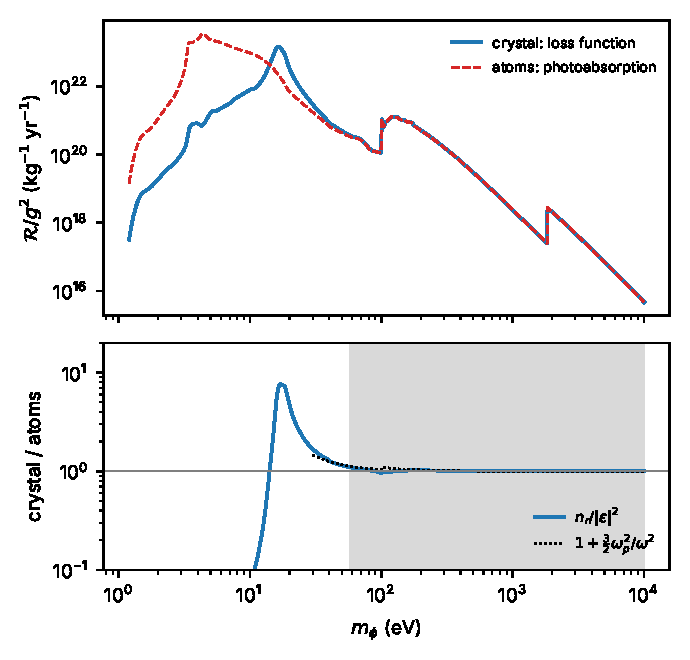
\includegraphics[width=0.92\linewidth]{figures/ch12/limit12_6a.pdf}
\captionof{figure}{Absorption of a scalar coupled equally to protons and neutrons ($c_\kappa = gA_\kappa$) in silicon against its mass $m_\phi$. Top: rate per unit mass divided by $g^2$, from the loss function, \cref{eq:12.6-absrate} (solid), and from the atomic formula with the measured photoabsorption of the crystal, $\nd_{\mathrm{at}}\sigma_\gamma = m_\phi\varepsilon_2/n_r$ (dashed); halo of \cref{sec:1.2}. Bottom: their ratio $n_r/|\varepsilon|^2$, with the expansion \cref{eq:12.6-medium} (dotted, $\omega_p$ from the electrons bound below $m_\phi$, binding energies of the $L$ and $K$ shells as in \cref{sec:10.6}). Dielectric function of silicon at \SI{300}{K}~\cite{franta2017temperature} below \SI{40}{eV} and from the atomic scattering factors~\cite{henke1993xray} above, as in \cref{sec:10.7}. Gray band: $m_\phi \ge \SI{57}{eV}$, where the atomic formula is within \SI{10}{\percent}.}\label{fig:12-limit-6a}
\par}
\smallskip
Below about \SI{60}{eV} the atomic formula misses the screening of the crystal, and is too high by about 400 near the absorption peak at \SI{4.2}{eV} and too low by 7.7 near the plasmon, at \SI{17}{eV}.
\end{limitbox}

\noindent On the truncation label \cref{lim:12.6a} sits at dipole order, $n_D = 2$ in the rate, with no Born--Oppenheimer truncation, since \cref{eq:12.6-accel,eq:12.6-mass} are exact; $\mathcal{X}$ is the measured loss function, and the lattice plays no role at these energies. Its next corrections are the multipoles of order $kr$, which at \SI{10}{keV} and a $1s$ radius of $a_0/Z$ are below $10^{-3}$, and, outside the shaded band, the full loss function in place of the atomic formula.

\emph{Couplings not proportional to mass.} If $c_\kappa/M_\kappa$ differs between species, write it as $\tilde c + \delta\tilde c_\kappa$, with $\tilde c$ a mean. The mean part is \cref{eq:12.6-absrate}. The remainder keeps the forces in \cref{eq:12.6-accel}, $\ii\omega^{-2}\sum_I\delta\tilde c_\kappa\,\vect{k}\cdot\langle f|\nabla_{\vect{X}_I}V|i\rangle$, and these no longer sum to anything simple. For transitions of the electrons the force on a nucleus is the density component of \cref{eq:12.1-force}, the vertex of the Migdal entry. The sum over the sites of one species, weighted by $\ee^{\ii\vect{k}\cdot\vect{X}_I}$, then forces the momentum given to the electrons to be $\vect{k} + \vect{G}$. The remainder is therefore a sum over reciprocal-lattice vectors weighted by the basis structure factor of $\delta\tilde c_\kappa Z_\kappa$, and it samples the off-diagonal elements $S^{ee}_{\vect{0}\vect{G}}$ and $S^{ee}_{\vect{G}\vect{G}'}$ of the electronic response at vanishing reduced momentum (\cref{eq:E.18-X}). These are nonadiabatic matrix elements in the sense of \cref{sec:12.1}: the response of the electrons to the force of one sublattice, which no optical measurement provides. For the core shells, which belong to one nucleus, the atomic dipole formula with $\delta\tilde c_\kappa$ in place of $\tilde c$ applies shell by shell. For the valence electrons \cref{app:E.18} specifies the calculation, with $S^{ee}_{\vect{G}\vect{G}'}$ to $|\vect{G}| = 6(2\pi/a)$ and the test that the (200) channel of the diamond structure vanishes for equal $\delta\tilde c_\kappa$. How large the remainder is depends on the coupling. For nucleon number in GaAs the two species differ in $A_\kappa/M_\kappa$ by $2.6\times10^{-5}$ per u (\cref{we:8-nucleon}), and the remainder is negligible. For a coupling to protons alone, $Z_\kappa/M_\kappa$ is 0.4446 per u for gallium and 0.4405 for arsenic, and the isotopes of natural silicon differ by up to \SI{7}{\percent}; the isotopic part is a random remainder, incoherent between sites, like the isotope scattering of \cref{sec:11.6}.

A scalar may also couple to electrons. Its amplitude adds $\tilde cm_e$ to the density coefficient $g^\phi_{n_e} = -g_{\phi ee}$ of \cref{eq:8.1-scalar}, and the kinetic row of the electron coupling, which dominates its absorption (\cref{sec:10.7}), interferes with the density row through their cross response. The nucleon coupling adds no new row.

\subsection{Nuisance table of the Migdal sector}\label{sec:12.6-table}

\Cref{tab:12-nuisances} collects the truncations and inputs of the chapter, each with its size and the section that treats it, in the classes of \cref{sec:8.8}.

\begin{table}[tbp]
  \caption{Nuisances of the Migdal sector. Type in the classes of \cref{sec:8.8}: normalization, tilt (in $\omega_e$, in $q$ or in the dark-matter mass), threshold and lattice spectrum (the share of a Migdal event that goes to phonons, at fixed electronic energy transfer). Basis of the size: ``computed'' (next order computed), ``model'' (next order computed in a model), ``est.''\ (parametric estimate), ``bound'' (only an inequality is known), ``named'' (no size). Sizes are for silicon unless another crystal is named. The last column gives the section where the item is treated.}
  \label{tab:12-nuisances}
  \centering\footnotesize\setlength{\tabcolsep}{3pt}
  \begin{tabular}{@{}>{\raggedright\arraybackslash}p{0.27\linewidth}>{\raggedright\arraybackslash}p{0.12\linewidth}>{\raggedright\arraybackslash}p{0.36\linewidth}>{\raggedright\arraybackslash}p{0.09\linewidth}>{\raggedright\arraybackslash}p{0.10\linewidth}@{}}
    \toprule
    Truncation or input & Type & Size & Basis & Section \\
    \midrule
    Local fields on the diagonal of $\varepsilon^{-1}$ (scalar $\varepsilon$ against $\varepsilon^{-1}_{\vect{G}\vect{G}}$) & normali\-zation; tilt in $\omega_e$ & factor 1.35 on the total, concentrated at $p \gtrsim q_{\mathrm{BZ}}$ (\cref{lim:12.3a}) & computed & \cref{sec:12.3} \\
    Off-diagonal elements $\vect{G} \neq \vect{G}'$ of $\varepsilon^{-1}$ & normali\-zation & raises the rate: full over diagonal 1.38 at $8^3$ points $\vect{k}$ and $|\vect{G}|^2 \le 19\,(2\pi/a)^2$, about 1.2 extrapolated, in an empirical-pseudopotential random-phase model of Si that carries about 2/3 of the diagonal local-field effect; still falling with $\vect{G}$, so the lower end is not a bound; flat in $\mchi$; the full local-field calculation is open; incoherent, zone-averaged form, not applicable at $q \ll q_{\mathrm{BZ}}$ & model & \cref{sec:12.1,sec:12.3} \\
    Loss-function table ($\omega_e \le \SI{89}{eV}$, $p \le \SI{22.5}{keV}$) & normali\-zation & $P_{\mathrm{Mig}}$: $\le\SI{1.6}{\percent}$ above \SI{89}{eV}; $p > \SI{10}{keV}$ holds \SI{2.3}{\percent}; drag mass: missing part $\le\SI{24}{\percent}$ & bound & \cref{sec:12.3,sec:12.5} \\
    Ion charge $Z_{\mathrm{ion}}(p)$ against a point ion & normali\-zation & $P_{\mathrm{Mig}}$ $\times1.57$; drag mass $18.6$ against $11.8\,m_e$ & model & \cref{sec:12.3,sec:12.5} \\
    Valence on-site drag mass & normali\-zation of the added lattice rate & Si $18.6\,m_e$ (12 to $24\,m_e$), Ge $39.5\,m_e$ (11.5 to $52\,m_e$); trace value $14\,m_e$ is not the on-site element & bound & \cref{sec:12.5} \\
    Per-mass form of the rate & tilt in $\mchi$ & within \SI{10}{\percent} above \SI{66}{MeV} & computed & \cref{sec:12.3} \\
    Frame of the transition density (lattice at $\vect{q} - \vect{p}$ or $\vect{q}$; Herzberg--Teller) & lattice spectrum & phonon-emitting fraction $\times2.4$ at \SI{5}{keV}; $+\SI{12}{\percent}$ in the displaced-oscillator model & model & \cref{sec:12.1,sec:12.4} \\
    Incoherent lattice factor below the zone & lattice spectrum & zero-phonon line within \SI{8}{\percent} of the Bragg sum; multiphonon terms uncertified below \SI{6.6}{keV} & computed; named & \cref{sec:12.4} \\
    Coherent zero-phonon response at $q < 2q_{\mathrm{BZ}}$ (cross-site terms of the lattice factor) & normali\-zation; tilt in $\omega_e$ & limit $q \ll q_{\mathrm{BZ}}$ (\cref{eq:8.3-boostward}): $1/14.9$ of the diagonal form, median $\omega_e$ \SI{17.4}{eV} against \SI{4.5}{eV}; within \SI{15}{\percent} only for $q \le \SI{0.75}{keV}$ (model), which carries $\le\SI{0.2}{\percent}$ of the rate at every mass; \SI{0.75}{keV} to $2q_{\mathrm{BZ}}$ unsized, nearly all of the rate up to \SI{1}{MeV}, \SI{33}{\percent} at 2 and \SI{7}{\percent} at \SI{3}{MeV} & computed (limit); model; unsized & \cref{sec:12.4} \\
    Exact energy denominators (recoil of $\vect{p}$, binding, Doppler; \cref{eq:12.3-bracket,eq:12.4-corr}) & tilt in $q$ & near the gap $-2.1\times10^{-3}$, $+2.8\times10^{-3}$ and at most $5.1\times10^{-4}$ below the impulse onset; free recoil: probability within \SI{10}{\percent} to $E_R \approx \SI{160}{eV}$, factor 1.6 at \SI{500}{eV}, rate within \SI{10}{\percent} to \SI{1}{GeV} & computed & \cref{sec:12.3,sec:12.4} \\
    Germanium lattice inputs (Debye-scaled) & lattice spectrum & $\langle\omega^{-1}\rangle^{-1} \approx \SI{17.6}{meV}$ from $\Theta_{\mathrm{D}} = \SI{373}{K}$; regime boundaries near 41 and \SI{113}{keV}; no first-principles phonon spectrum & est. & \cref{sec:12.4} \\
    Dipole order of the atomic boost (cores) & tilt in $q$ & within \SI{10}{\percent} to $\xi_D = 0.188$ (Si), 0.127 (Ge) & computed & \cref{sec:12.2} \\
    Bound final states of the atom & normali\-zation & lower bound only & bound & \cref{sec:12.2} \\
    Wannier picture of the boost & normali\-zation & absolute bound 1.6, 0.54, 0.25 at 20, 50, \SI{100}{eV}; non-rigid ratio open & bound & \cref{sec:12.3} \\
    Relativistic contact density (third moment) & normali\-zation of the check & $+\SI{8}{\percent}$ (Si), $+\SI{42}{\percent}$ (Ge); non-logarithmic Dirac remainder and $p_{1/2}$ contact density uncontrolled, each of relative order $(Z\alpha)^2$ (\SI{5}{\percent} in Ge) & computed; est. & \cref{sec:12.5} \\
    Site difference of $Z^*_\kappa(\omega)$, GaAs bremsstrahlung & normali\-zation & $-19$ to $+\SI{25}{\percent}$ at \SI{100}{MeV} & bound & \cref{sec:12.6} \\
    Atomic formula for Migdal-type absorption & tilt in $m_\phi$ & within \SI{10}{\percent} above \SI{57}{eV}; about $400\times$ high at \SI{4.2}{eV} & computed & \cref{sec:12.6} \\
    Couplings not proportional to mass & normali\-zation & Umklapp remainder (\cref{eq:E.18-X}) & named & \cref{sec:12.6} \\
    \bottomrule
  \end{tabular}
\end{table}

For the silicon Migdal probability above a few MeV the table has one large computed row, the local fields on the diagonal, and one large row sized only in a model, the off-diagonal part, which acts in the opposite direction. The table truncation, by contrast, costs a few percent, and the ion charge is fixed by the frozen core. The per-mass form is not an uncertainty of a correct calculation but the error of a simpler one, and its size says where the simpler one may be used. The counting of Migdal and lattice events depends on the on-site drag mass, which is known only within a factor of two. And the frame of the transition density changes how a Migdal event shares its energy between electrons and lattice without changing how many events there are, which matters to a detector that reads both charge and phonons.

\subsection{Open problems}\label{sec:12.6-open}

The dynamical Born charges of a polar crystal are fixed by \cref{eq:12.6-sum} only in their sum; the difference between the sites needs the frequency-dependent calculation of \cref{app:E.17}, and until it is done the GaAs bremsstrahlung rate carries the band of \cref{fig:12-brems}. And the absorption of a scalar whose couplings are not proportional to the masses needs the off-diagonal response $S^{ee}_{\vect{G}\vect{G}'}$ at vanishing reduced momentum, which \cref{app:E.18} specifies. The open items of the earlier sections are rows of \cref{tab:12-nuisances}. Above all of them stands a measurement. No crystal Migdal signal has yet been observed. A tagged-recoil measurement, in which the energy and direction of each nuclear recoil are fixed independently, for instance by the kinematics of a neutron scattered at a known angle, and the electrons it releases are counted, would test the whole chain at once in silicon at the recoil energies of \cref{sec:12.5}.

\section*{Summary}

A kicked nucleus leaves energy in two places, the lattice and the electrons, and the joint response resolves the two (\cref{sec:12.1}). It is the response of \cref{sec:8.7} sorted by the electronic energy transfer $\omega_e$ and the lattice energy $\omega_l$; its marginal is the ordinary response, and the sectors of \cref{sec:8.6} fall on the two axes and the quadrant between them. At the leading nonadiabatic order its Migdal entry is the response of the electrons to the field of a suddenly moving nucleus: a boost $\vect{q}\cdot\vect{p}/M_\kappa\omega_e^2$, the bare vertex of the nucleus, the density response of the clamped electrons and the lattice response at the momentum the nucleus keeps. The four published Migdal formulas are truncations of that entry. Its first moment is fixed by the drag mass, and the estimate $P_{\mathrm{Mig}} \approx (E_R/\langle\omega_e\rangle)(\delta M_\kappa/M_\kappa)$ follows. Added to a lattice rate, a Migdal rate requires the lattice response with the weight $1 - P_{\mathrm{Mig}}$ and the dragged mass, and a measured nuclear-recoil yield already contains the Migdal ionization. In a metal the sudden expansion fails at small $\omega_e$.

The isolated atom is the truncation in which the boost can be done to all orders (\cref{sec:12.2}). The center of mass separates exactly, and the electrons receive the momentum $m_e\vect{q}/m_A$, with $m_A$ the mass of the whole atom. At dipole order the ionization probability at a recoil energy of \SI{1}{keV} is $2.09\times10^{-3}$ for silicon and $1.63\times10^{-3}$ or $1.73\times10^{-3}$ for germanium in two independent calculations, and the dipole form holds within \SI{10}{\percent} up to $\xi_D = 0.188$ and 0.127. Bound final states without ionization add to it, and the oscillator strengths give only a lower bound on their share. In a crystal the atomic form is the right one for the core shells, not for the valence.

At large momentum transfer the crystal Migdal probability is a weighted moment of the loss function, with the coefficient $4\alpha$ fixed by the $f$-sum rule and the valence ionization factor $Z_{\mathrm{ion}}(p)$ in the vertex (\cref{sec:12.3}). In silicon it is $6.1\times10^{-5}$ per eV of recoil energy, 29 times the atomic value. A scalar dielectric function overestimates it by about \SI{35}{\percent}, an error concentrated at $p \gtrsim q_{\mathrm{BZ}}$; the off-diagonal elements of the dielectric matrix raise it in a model by a factor of about 1.4 as computed and 1.2 extrapolated, the lower end not a bound, and their full calculation is open. The soft limit has no correction in $p/q$ and holds at low mass; it fails only when the nucleus moves fast during the transition, above about \SI{160}{eV} of recoil. The factorized rate per unit mass holds within \SI{10}{\percent} above \SI{66}{MeV}. The Wannier picture of the boost is exact for flat bands and bounded only in absolute terms for the valence band of silicon.

Below the impulse onset the lattice factor of the Migdal entry is the multiphonon response at the momentum the nucleus keeps (\cref{sec:12.4}). The electronic spectrum does not depend on it, since the lattice factor has unit weight. What it decides is how a Migdal event shares its energy: at \SI{10}{keV} in silicon \SI{92}{\percent} of the events leave the lattice in its ground state, and most events stay zero-phonon until the zero-phonon weight of the kick itself falls to one half, at \SI{33.2}{keV}. The phonon-mediated form is the same process with the bound-nucleus propagator, exact in the phonon energies at first order in $\vect{p}$; for silicon and germanium its correction is a few parts in a thousand at the gap, and it matters only where gaps approach phonon energies.

The moments of the Migdal spectrum are inverse moments of the force that the electrons exert on one nucleus (\cref{sec:12.5}). The first is the on-site drag mass, which differs from the trace value of $14\,m_e$ for silicon that a uniform translation fixes; the loss function gives $18.6\,m_e$ for the valence electrons alone, uncertain by a factor of two. Two moments bound the probability from both sides. The cross first moment fixes the Migdal interference of a mixed coupling, and the third moment is the electron density at the nucleus, which relativity raises by \SI{8}{\percent} in silicon and \SI{42}{\percent} in germanium.

A recoiling nucleus also radiates, and an absorbed scalar coupled to nucleons gives its energy to the electrons through the same boost (\cref{sec:12.6}). The crystal emits with the dynamical Born charge, which in silicon and germanium follows exactly from the measured dielectric function and suppresses the emission as the fourth power of the photon energy. Silicon still emits 33 to 38 times more than its atoms, and GaAs, with its static Born charge, $1.87\times10^4$ times more over its transparent band. The rates are seven orders below the Migdal rate, so bremsstrahlung is a check, not a channel. A scalar whose couplings to the nuclei are proportional to their masses is absorbed with the loss function, by the equivalence principle, and the atomic formula holds in silicon only above \SI{57}{eV}. The chapter's nuisances are collected in \cref{tab:12-nuisances}. Throughout, the electronic final states were reached by kicking a nucleus; \cref{chap:13} turns to the other mixed sector, the electrons kicked directly while a phonon carries the missing momentum.
